\documentclass{article}
\usepackage[margin=1in]{geometry}
\usepackage{amsmath,amsthm,amssymb}
\usepackage{bbm,enumerate,mathtools}
\usepackage{tikz,pgfplots}
\usepackage{chessboard}
\usepackage[hidelinks]{hyperref}
\usepackage{multicol} % Problem 35

\newenvironment{question}{\begin{trivlist}\item[\textbf{Question.}]}{\end{trivlist}}
\newenvironment{note}{\begin{trivlist}\item[\textbf{Note.}]}{\end{trivlist}}
\newenvironment{references}{\begin{trivlist}\item[\textbf{References.}]}{\end{trivlist}}
\newenvironment{related}{\begin{trivlist}\item[\textbf{Related.}]\end{trivlist}\begin{enumerate}}{\end{enumerate}}


\begin{document}
\rating{2}{4}

Richard Stanley guesses that determining whether or not an arbitrary polyomino can be used to tile a rectangle is undecidable---that is, there is not a general purpose algorithm that can do so. We call such polyominoes ``rectifiable.''

Here we define something different: we say that a polyomino is ``toroidal'' if it can be used to tile a rectangular torus grid. All rectifiable polyominoes are toroidal, and all polyominoes that tile the plane with two dimensions of translational symmetry are toroidal.

\begin{figure}[ht!]
  % 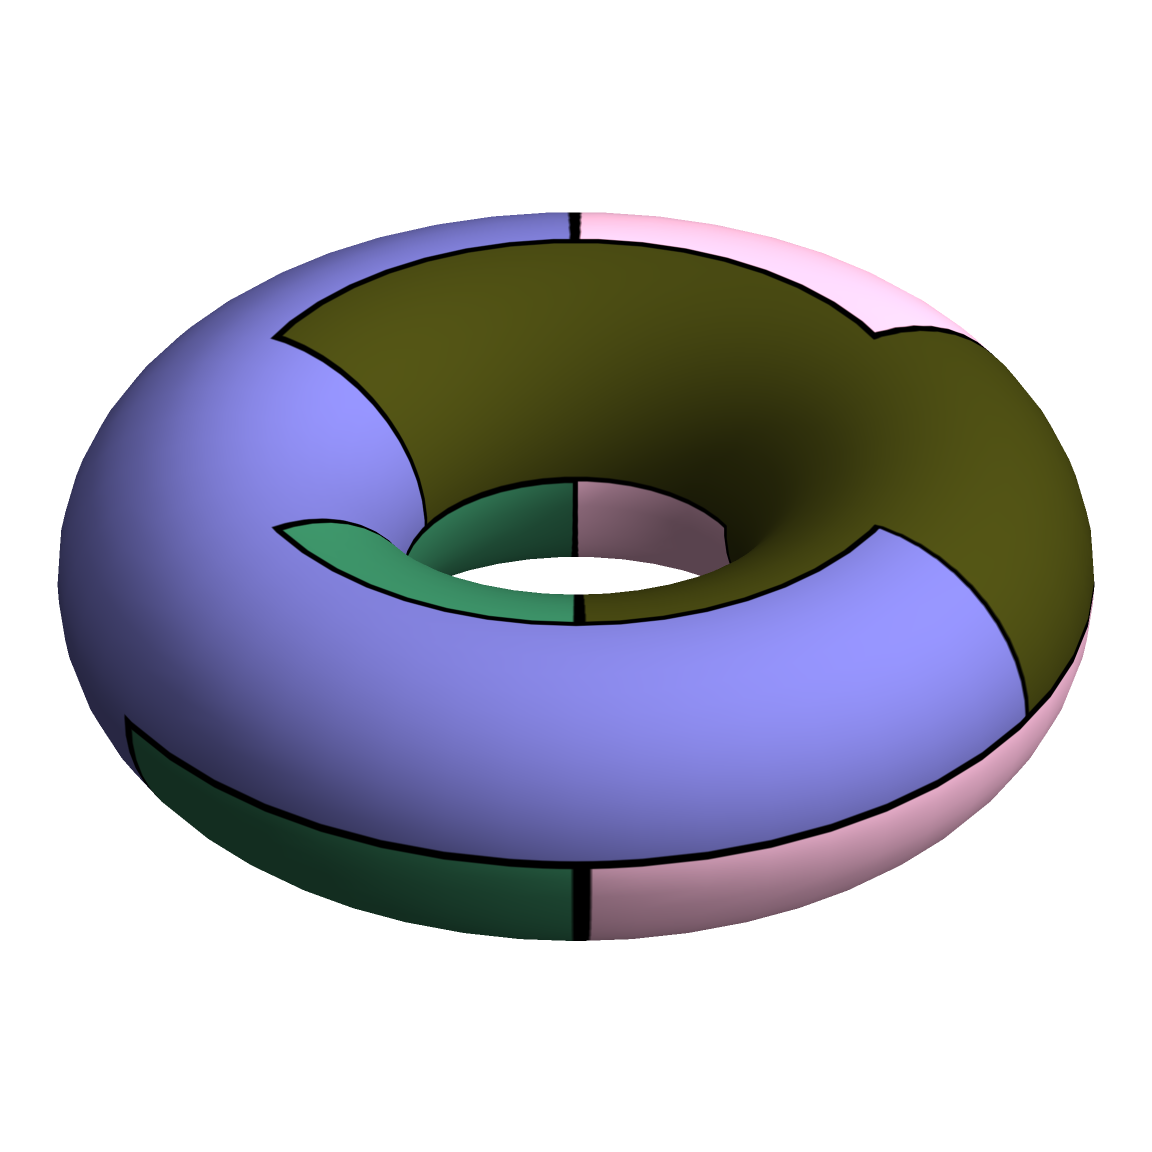
\includegraphics[width=0.3\linewidth]{assets/138_problem/embedded_torus.png}
  \begin{tikzpicture}
    \node at (0,0) {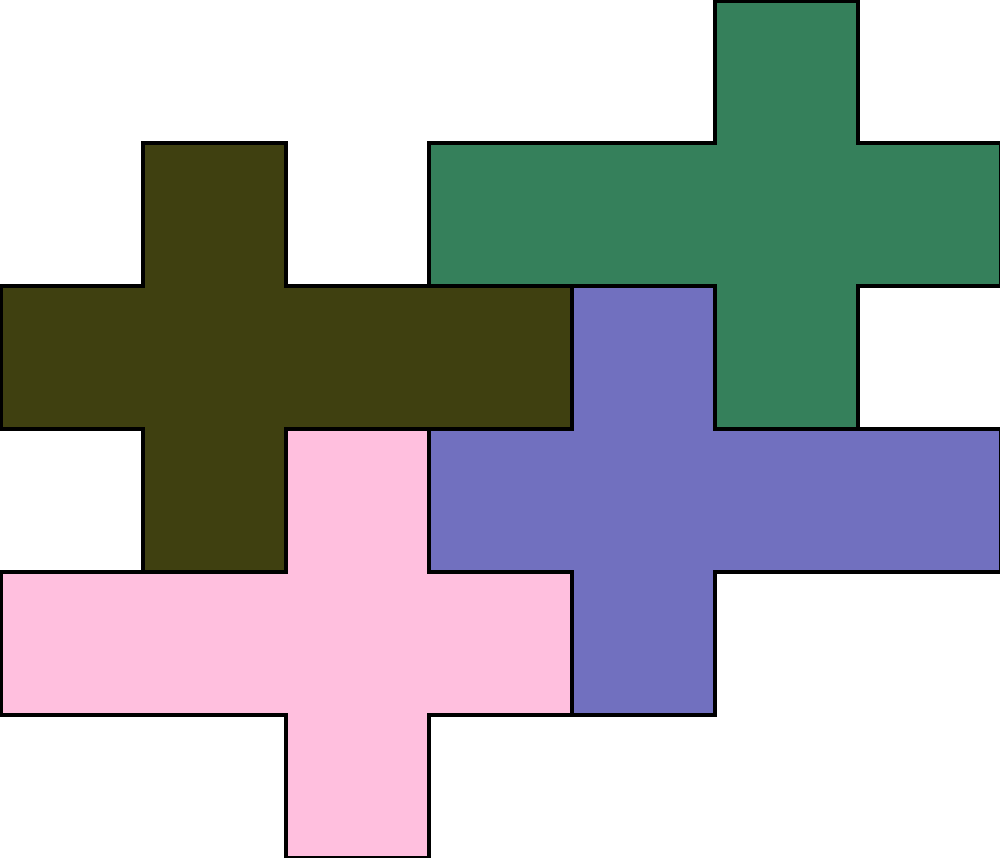
\includegraphics[width=0.3\linewidth]{assets/138_problem/unfolded.png}};
    \node at (5.5,0) {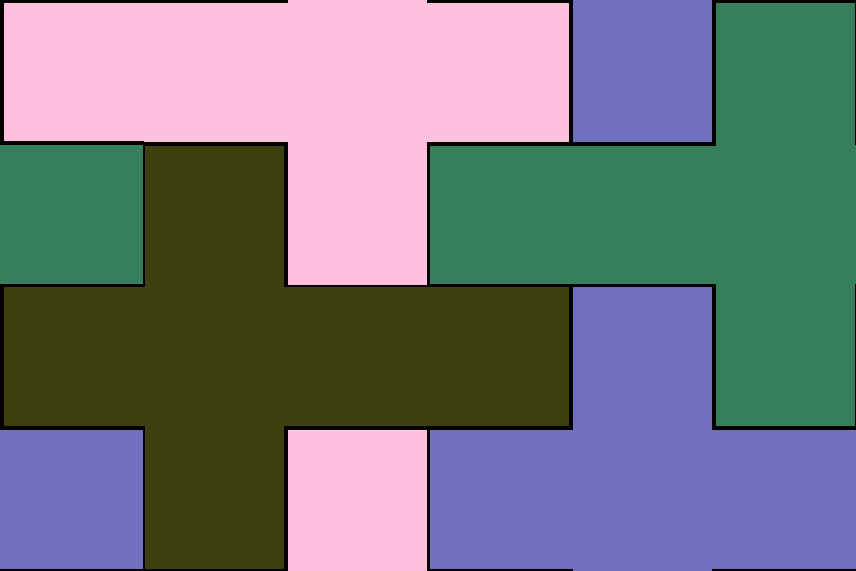
\includegraphics[width=0.257\linewidth]{assets/138_problem/flat_torus.png}};
    \draw[thick] (7.6,-1.4) rectangle (3.4,1.4);
    \draw[red,line width=3, ->] (3.4,-1.4) -- (5.5,-1.4);
    \draw[red,line width=3, ->] (3.4,-1.4) -- (6,-1.4);
    \draw[red,line width=3] (3.4,-1.4) -- (7.6,-1.4);
    \draw[red,line width=3, ->] (3.4,1.4) -- (5.5,1.4);
    \draw[red,line width=3, ->] (3.4,1.4) -- (6,1.4);
    \draw[red,line width=3] (3.4,1.4) -- (7.6,1.4);

    \draw[blue,line width=3, ->] (3.4,-1.4) -- (3.4,0.2);
    \draw[blue,line width=3] (3.4,-1.4) -- (3.4,1.4);
    \draw[blue,line width=3, ->] (7.6,-1.4) -- (7.6,0.2);
    \draw[blue,line width=3] (7.6,-1.4) -- (7.6,1.4);

    \node at (11,0) {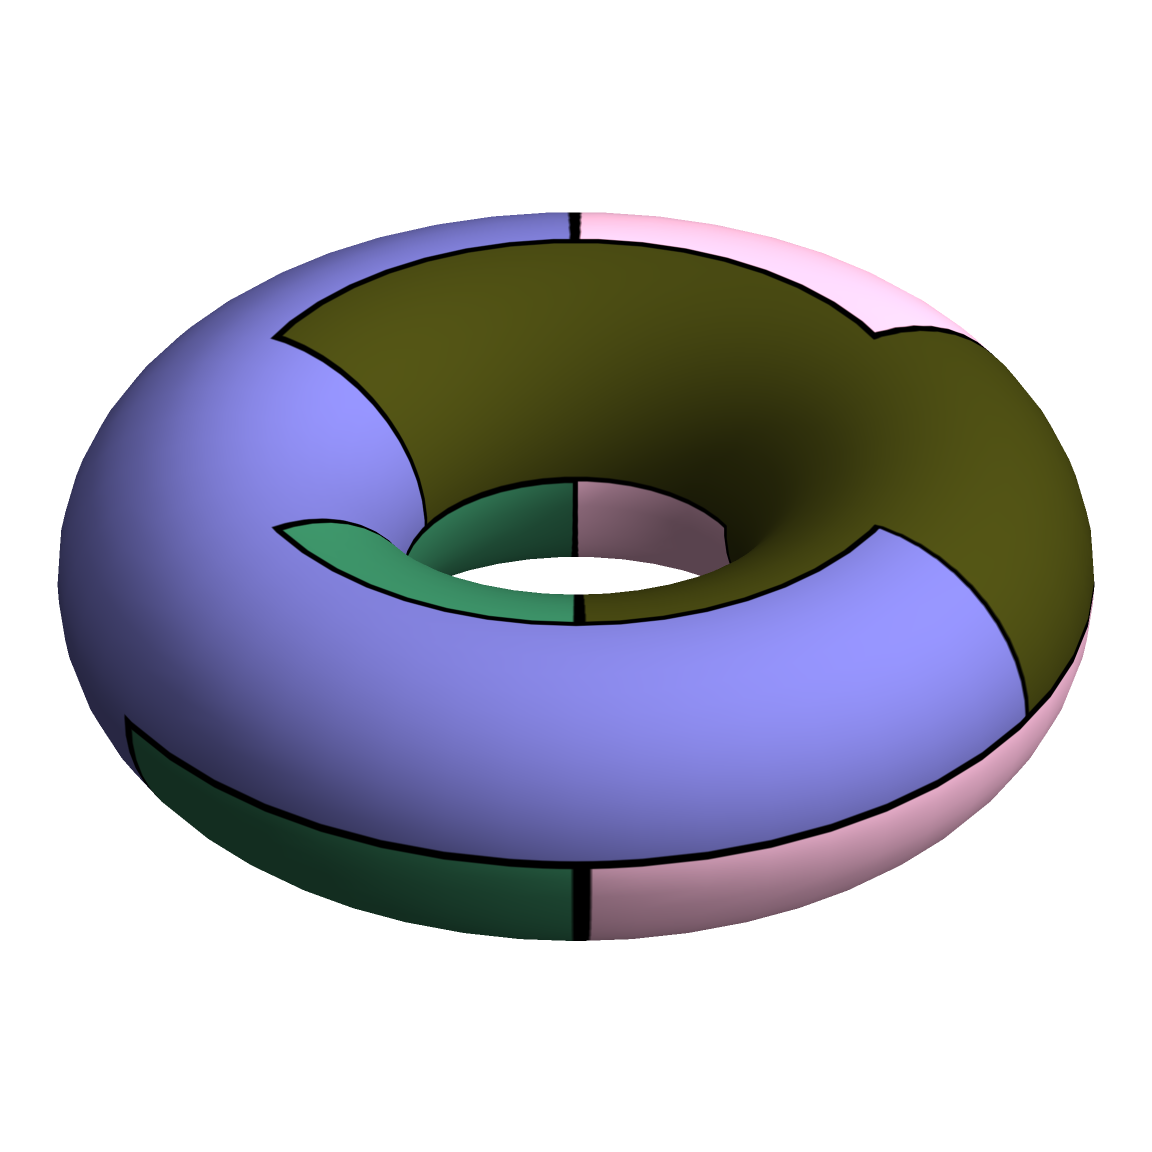
\includegraphics[width=0.3\linewidth]{assets/138_problem/embedded_torus.png}};
\end{tikzpicture}
  \caption{
    An illustration of a toroidable $6$-omino that is not rectifiable.
  }
\end{figure}

\begin{question}
  For each $n$, what is the toroidable $n$-omino with the largest minimal torus?
\end{question}

\begin{related}
  \item What about polyiamonds? Polyhexes? Other polyforms?
  \item Suppose we want to $k$-color the torus so that no color is adjacent to itself by an edge (alternatively, vertex). What is the largest minimal coloring over all $n$-ominoes.
\end{related}

\begin{references}
  \item MathOverflow.
\end{references}
\end{document}
